{
  \newcommand{\colorgradientbox}{%
    \tikz[baseline=-0.5ex]{
      \node[minimum height=1em, minimum width=3em, draw=black, line width=0.8pt,
            shading=horizontal, left color=white, right color=red] (char) {};
    }\;%
  }

  \newcommand{\solidcolorbox}{%
    \tikz[baseline=-0.5ex]{
      \node[minimum height=1.0em, minimum width=1.0em, draw=black, line width=0.8pt, fill=green!20!white] (char) {};
    }\;%
  }

  \begin{figure}[h]
      \centering
      \begin{subfigure}{.33\textwidth}
          \centering
          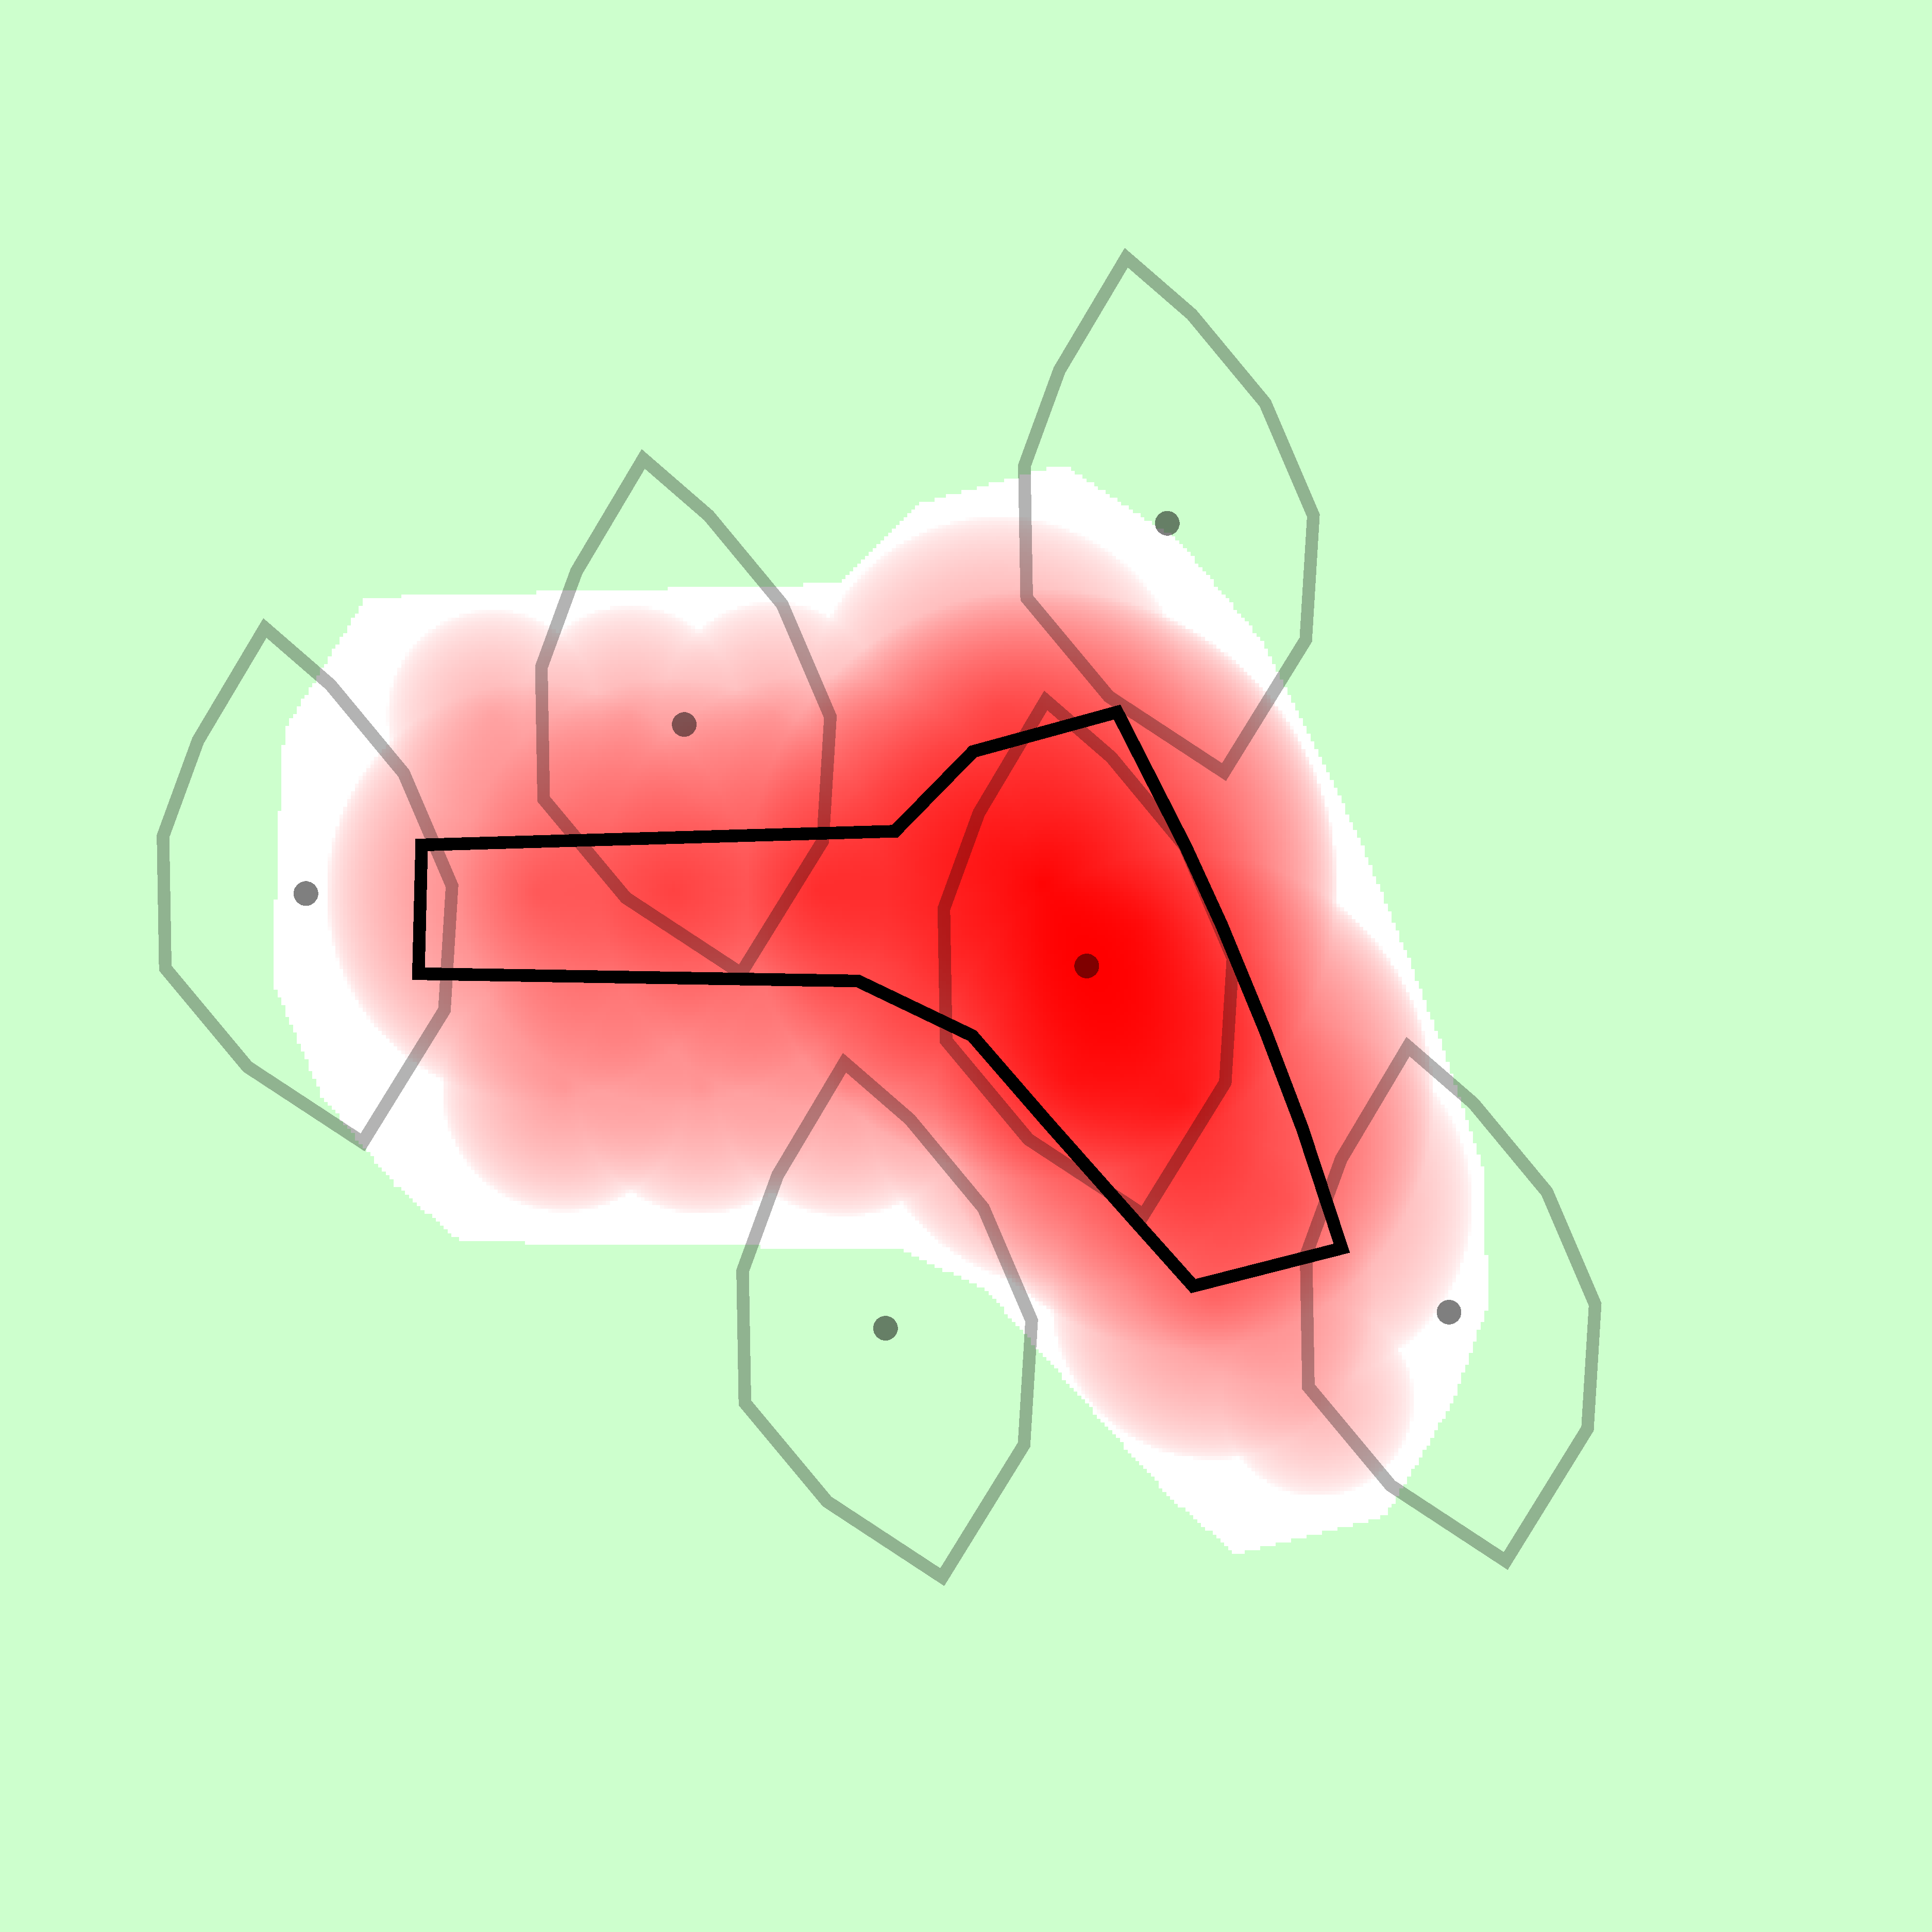
\includegraphics[trim={60 100 220 180}, clip=true, width=1.0\textwidth]{overlap_no_decay.svg.pdf}
          \caption{2D}
          \label{fig:overlap_no_decay_2d}
      \end{subfigure}
      \hspace{0.1\textwidth}
      \begin{subfigure}{.33\textwidth}
          \centering
          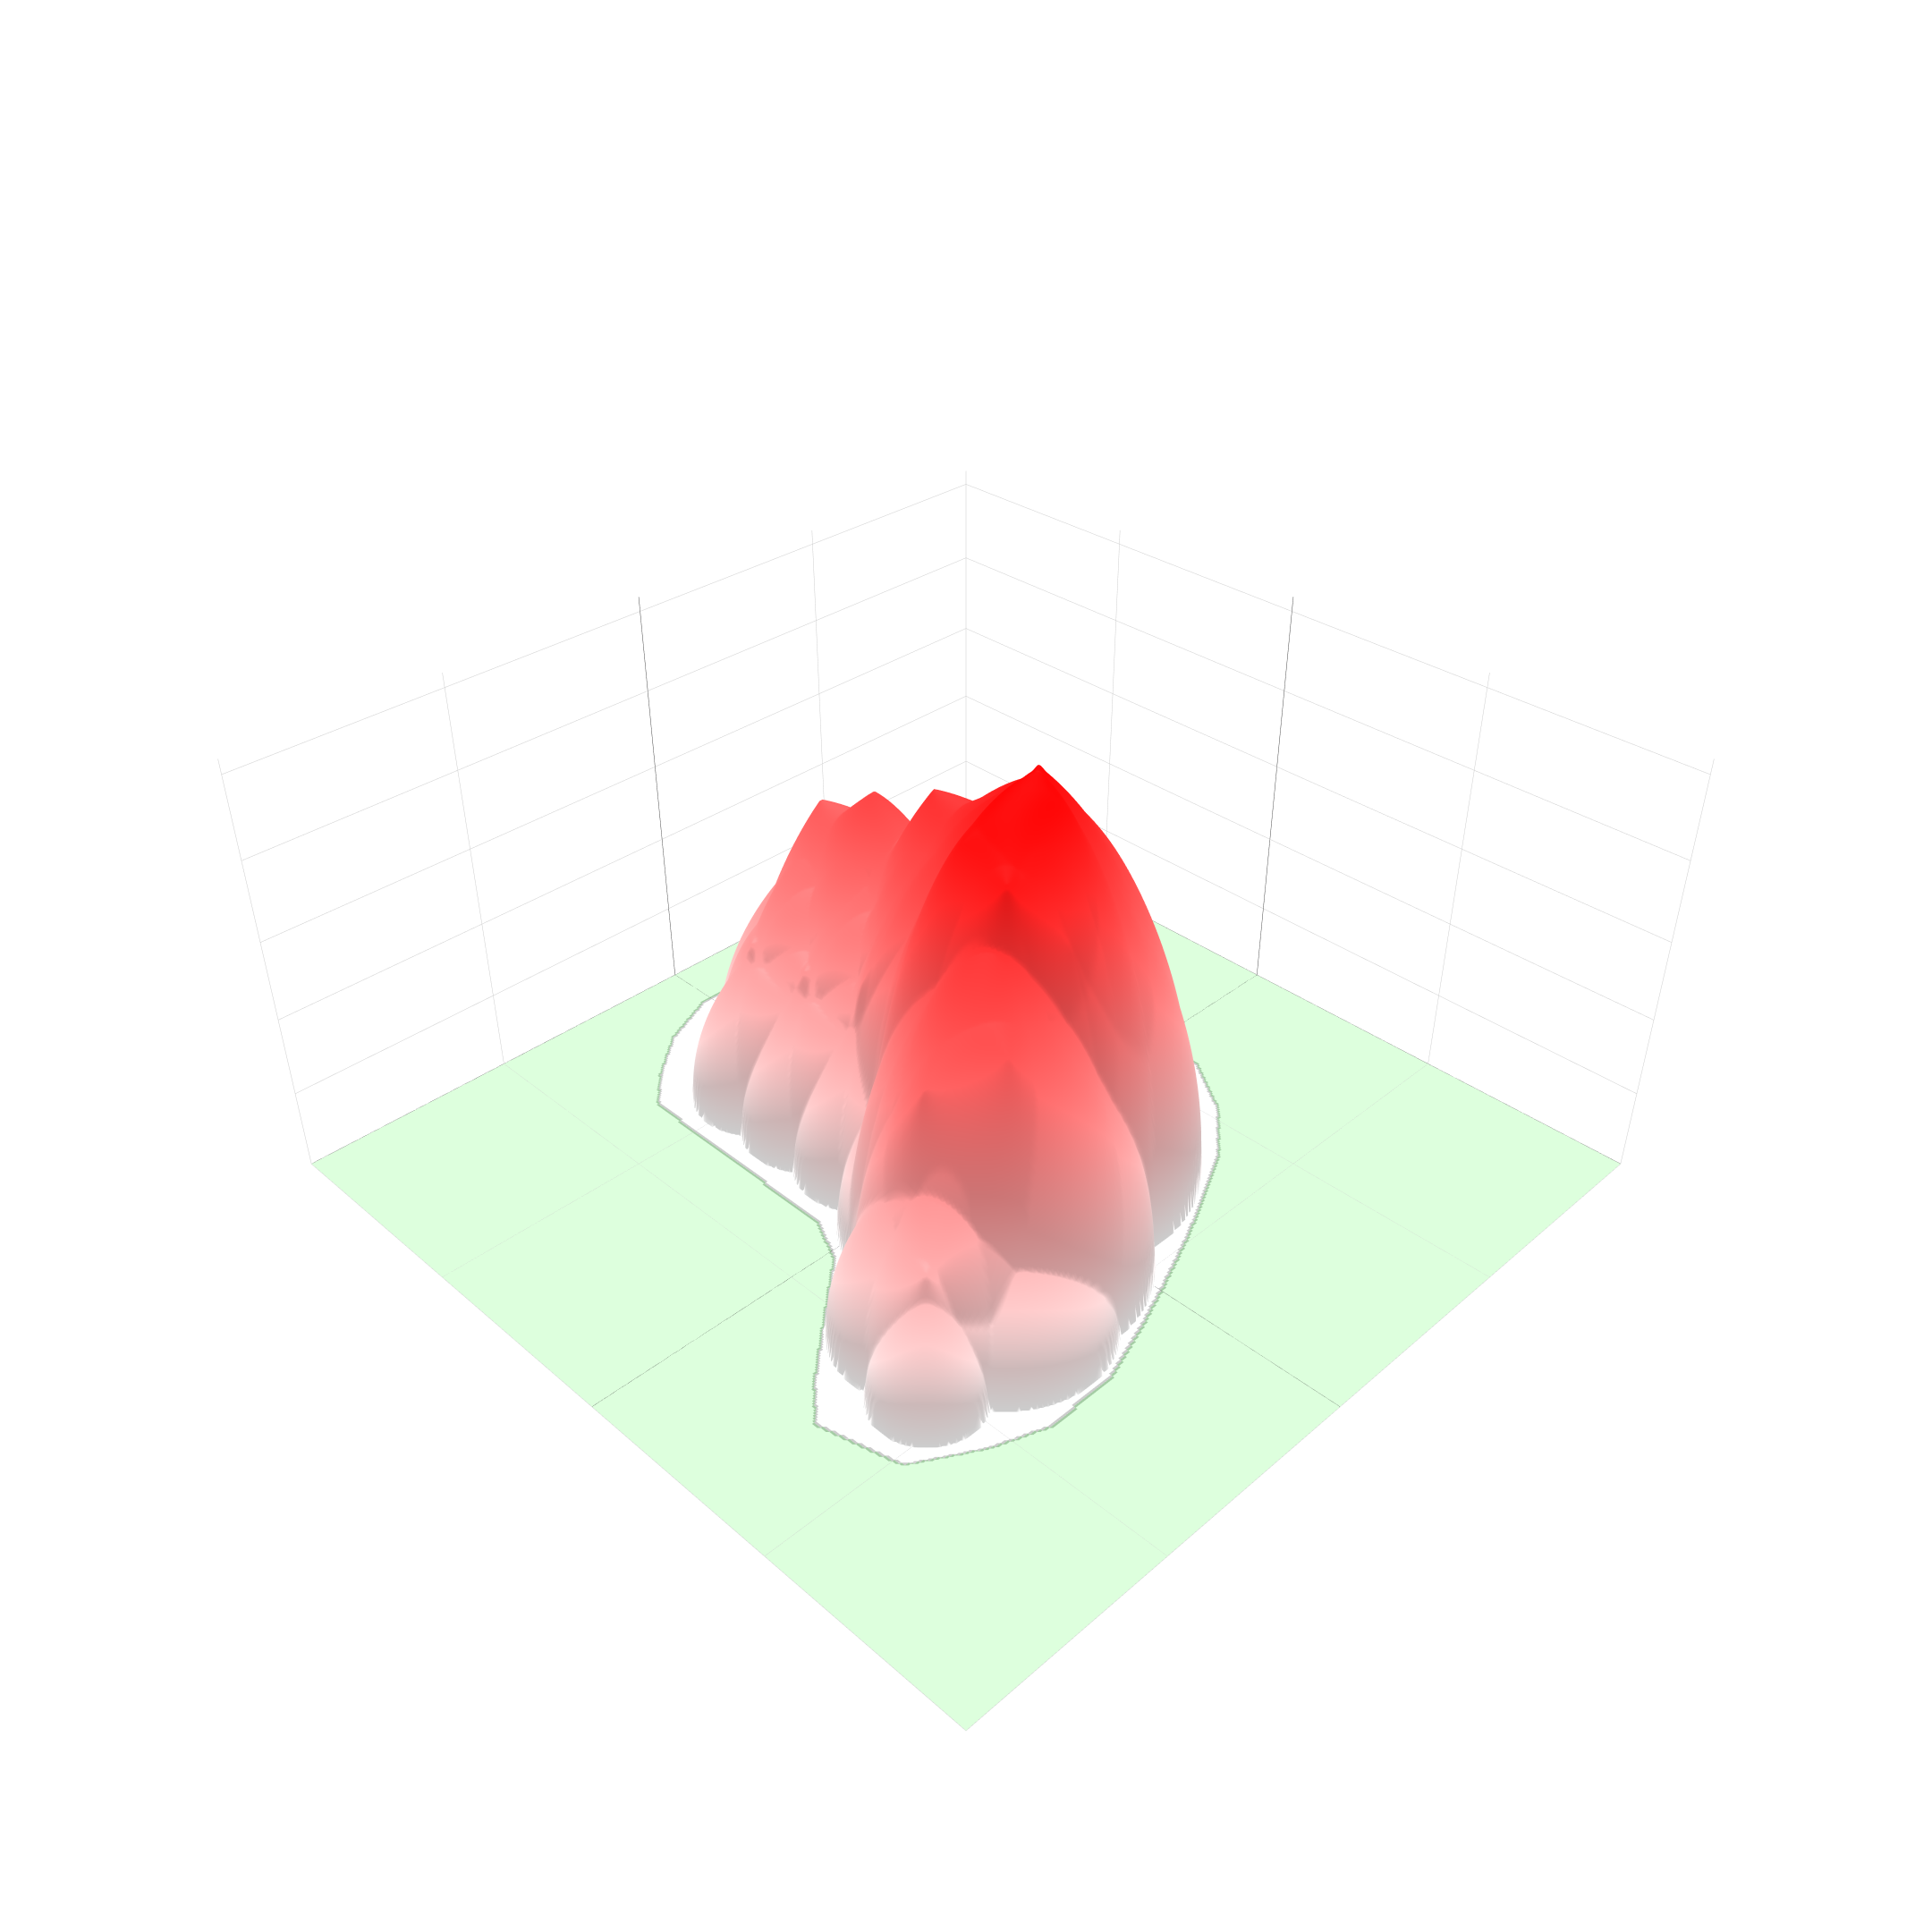
\includegraphics[trim={600 400 600 800}, clip=true, width=1.0\textwidth]{overlap_3d_no_decay.png}
          \caption{3D}
          \label{fig:overlap_no_decay_3d}
      \end{subfigure}
      \caption{Visualization of the overlap proxy for the same pair of items from Figure~\ref{fig:poles}.
      {\protect\solidcolorbox}: feasible, {\protect\colorgradientbox}: \nameref{alg:overlap_area_proxy}.}
      \label{fig:overlap_no_decay}
  \end{figure}
}